\documentclass[11pt,a4paper,compress]{beamer}%,handout
\usepackage[utf8]{inputenc}
\usepackage[english]{babel}
%\usepackage{varioref}
\usepackage{xspace}
\usepackage{ucs}
%\usepackage{eurosym}
\usepackage{graphicx}
%\usepackage{color}
%\usepackage{tikz-timing}
\usepackage{multicol}
%\usepackage[x11names]{xcolor}
\usepackage{colortbl}
%\usepackage{hyperref}
%\usetheme{Luebeck}
%\usetheme{Warsaw}
%\usetheme{Copenhagen}
\usepackage{fontawesome}

%\usetheme{Luebeck}%Madrid
\usetheme{default}%Madrid
\usecolortheme{whale}
\usecolortheme{orchid}
%\useinnertheme{default}%dirty hack to suppress the shadow on the background gradient
\useoutertheme{infolines}



\usepackage{pgfpages}
%\pgfpagesuselayout{4 on 1}[a4paper,landscape,border shrink=5mm,border code=\pgfstroke]



\makeindex

\title[]{ELEC-H-473 Microprocessor Architectures\\%Présentation\\
$\sim$ \\
\large
Short introduction to the labs
}
\institute[\begin{tiny}ULB--BEAMS\end{tiny}]{%ULB--BEAMS%

\includegraphics[height=1.1cm, origin=c]{figures/ulbquadri_mini.pdf} ~~ 
\includegraphics[height=1cm, origin=c]{figures/beamsWODept.pdf} ~~\raisebox{-2mm}{} %\includegraphics[height=0.75cm]{ee_Xlarge.png}
% \\ $\therefore$ \\ \includegraphics[height=0.75cm]{inpn7logo.pdf}
 }%{BEAMS - ULB\\  ENSEEIHT}

\date[]{}

\setcounter{tocdepth}{3}


\makeatletter
\defbeamertemplate{itemize item}{myball}%
{\raise-0.2cm\hbox{\Large\insertenumlabel.}}
\makeatother

\definecolor{orange}{RGB}{255,223,138}
\definecolor{red}{RGB}{255,200,200}
\definecolor{redred}{RGB}{255,00,00}
\definecolor{green}{RGB}{8,201,27}
\useinnertheme{rounded}
\useinnertheme{default}
\useinnertheme{circles}
\begin{document}

\setbeamertemplate{footline}% from {infolines theme}
{
  \leavevmode%
  \hbox{%
  \begin{beamercolorbox}[wd=.5\paperwidth,ht=3.25 ex, dp=1 ex, center]{author in head/foot}%
    \usebeamerfont{author in head/foot}\insertshortinstitute%\insertshortauthor~~%\insertshortinstitute
  \end{beamercolorbox}%
  %\begin{beamercolorbox}[wd=.333333\paperwidth,ht=2.25 ex, dp=1 ex,center]{title in head/foot}%
  %  \usebeamerfont{title in head/foot}%\insertshortinstitute
  %\end{beamercolorbox}%
  \begin{beamercolorbox}[wd=.5\paperwidth,ht=3.25 ex, dp=1 ex,right]{date in head/foot}%
    \usebeamerfont{date in head/foot}\hspace*{2 em}
    {\small \textbf{\insertframenumber{}}} \hspace*{2 ex}
  \end{beamercolorbox}}%
 % \vskip1pt%
}


\setbeamertemplate{navigation symbols}{}
\setbeamertemplate{itemize item}[default]
\setbeamertemplate{itemize subitem}[default]
\setbeamerfont*{itemize/enumerate body}{size=\large}
\setbeamerfont*{itemize/enumerate subbody}{parent=itemize/enumerate body}
\setbeamerfont*{itemize/enumerate subsubbody}{parent=itemize/enumerate body}


\begin{frame}[plain]
	\titlepage

\end{frame}



\section{Introduction}
\AtBeginSection[] % Do nothing for \section*
{
	% \frame<beamer>
	% {
	% 	\frametitle{Plan}
	% 	\tableofcontents[currentsection, hidesubsections, hideallsubsections ]%
	% }
}

\AtBeginSubsection[] % Do nothing for \subsection*
{
}
\setcounter{tocdepth}{1}
\begin{frame}
\frametitle{Practical discovery of microprocessors}
\begin{center}
\only<1>{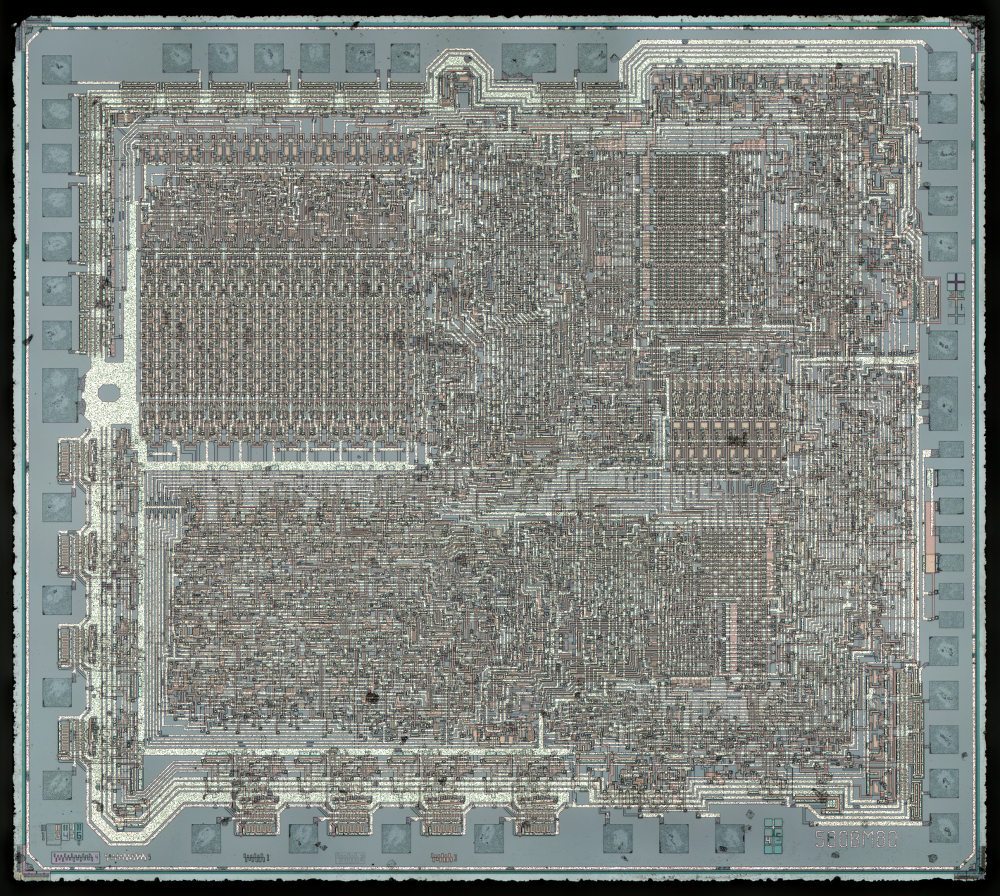
\includegraphics[width=7cm]{figures/kr580vm80a-2.jpg}}
\only<2>{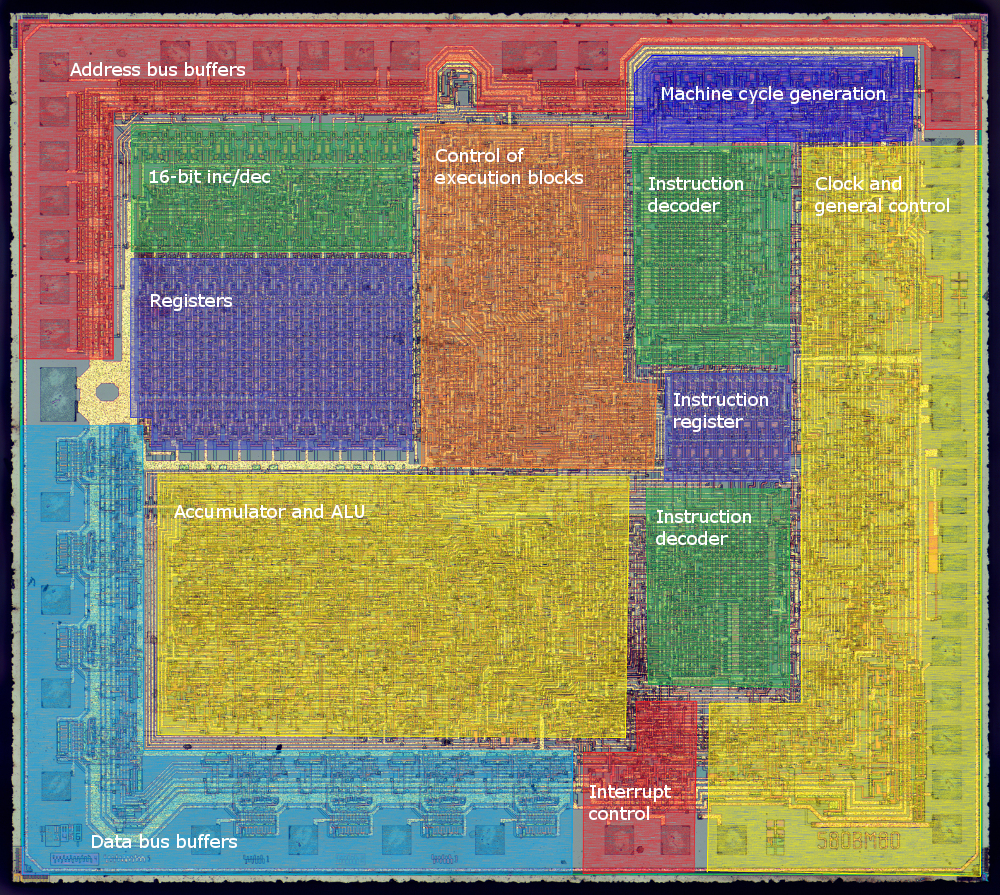
\includegraphics[width=7cm]{figures/kr580vm80a-annotation.jpg}}
\end{center}
KR580VM80A die shot, CC by http://zeptobars.ru
\end{frame}
\begin{frame}
\frametitle{}
%\begin{block}<+->{
\begin{center}
{\Huge How does it work, for real ?}
\end{center}
%}\end{block}

\end{frame}

\begin{frame}
	\frametitle{Plan}
	\tableofcontents[hidesubsections]
\end{frame}
\setcounter{tocdepth}{3}

\section{The UA5 lab}
\begin{frame}
\frametitle{The UA5 lab}
%Voiture shadok

\begin{block}<+->{If you are not (yet) familiar with this lab:}

\begin{itemize}
%\item Allumage des clignotants
\item This is not a restaurant: no food
\item This is not a bar: no drinks (except closed bottles)
\item Keep quiet, people are thinking hard here
%\item Attendance is mandatory
\item Keep the room tidy
%\item GPS
\end{itemize}
\end{block}
\end{frame}

\begin{frame}
\frametitle{People involved}
\begin{itemize}
\item Dragomir Milojevic\\
\begin{center}
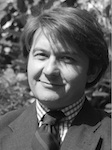
\includegraphics[height=2cm]{figures/d.jpg}
\end{center}
\end{itemize}

\begin{minipage}[t]{0.3\linewidth}
\begin{itemize}
\item Ken\\ Hasselmann
\begin{center}
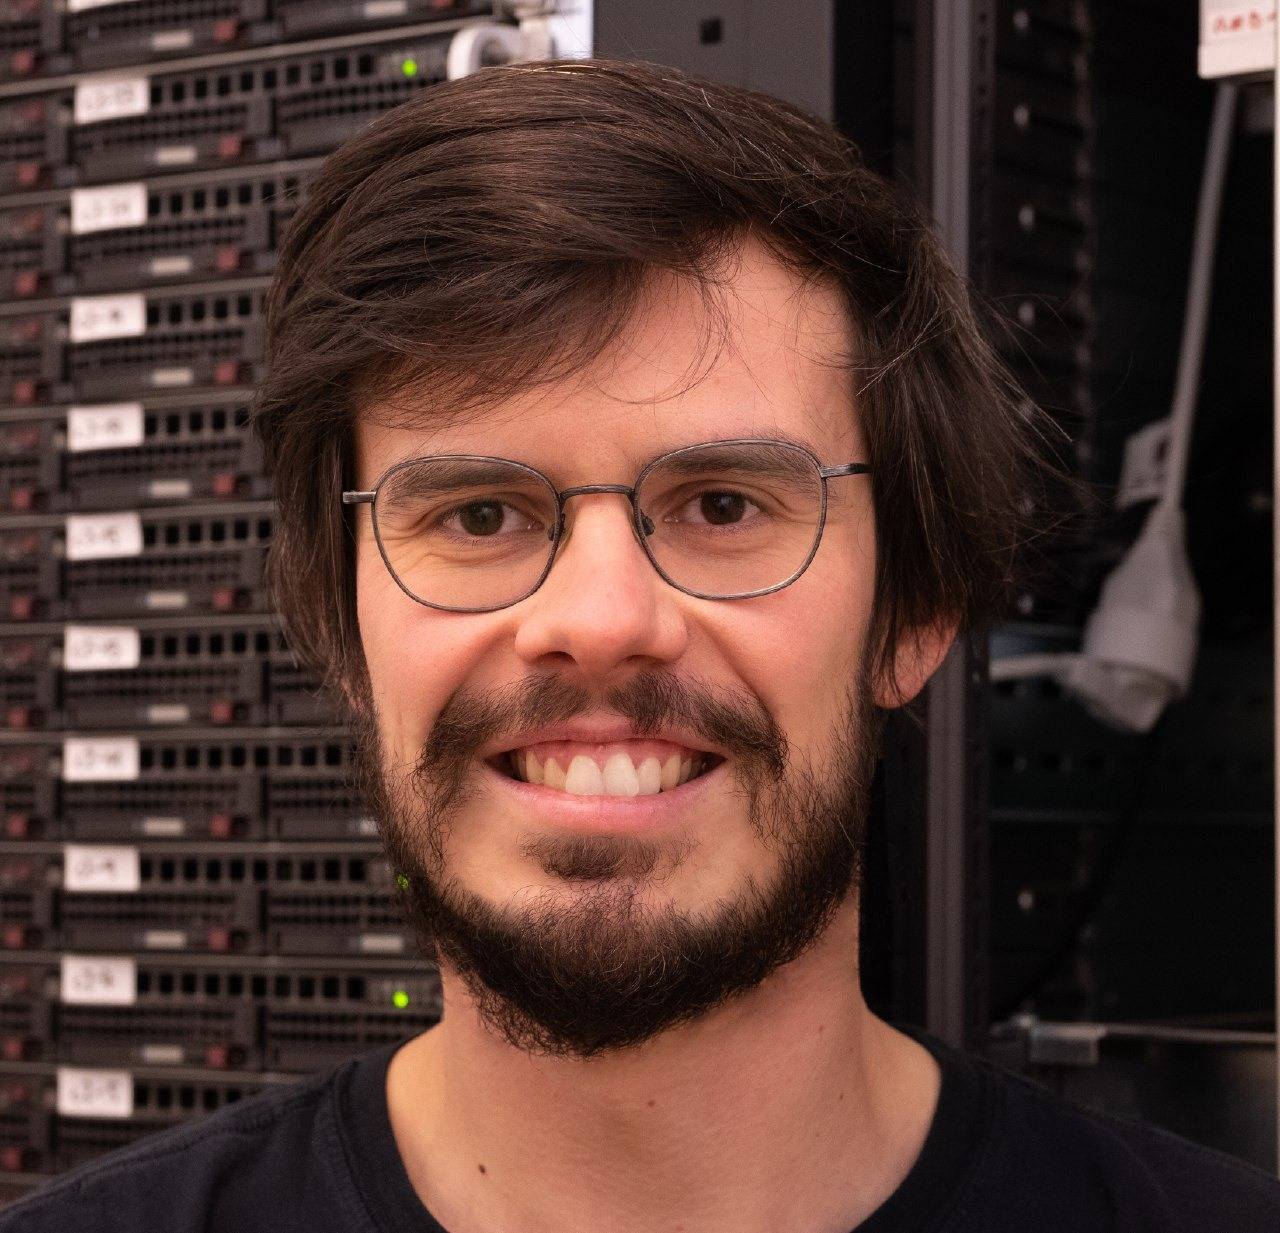
\includegraphics[height=2cm]{figures/k.jpg}
\end{center}
\end{itemize}
\end{minipage}
%
\begin{minipage}[t]{0.3\linewidth}
\begin{itemize}
\item Quentin\\ Delhaye
\begin{center}
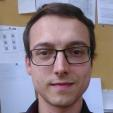
\includegraphics[height=2cm]{figures/QD.jpg}
\end{center}
\vspace{2.3cm}
\end{itemize}
\end{minipage}
%
\begin{minipage}[t]{0.3\linewidth}
\begin{itemize}
\item Cédric\\ Hannotier
\begin{center}
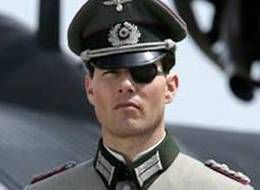
\includegraphics[height=2cm]{figures/c.jpg}
\end{center}
\vspace{2.3cm}
\end{itemize}
\end{minipage}

\end{frame}

\section{The labs}
\begin{frame}
\frametitle{The labs}

3 microprocessor architectures:
\begin{itemize}
\item RiSC16: Very small RISC, 4 labs
\item[]
\item dsPIC33: Microcontroller, also RISC, 1 lab
\item TIS-100, 1 lab
\item[]
\item x86\_64: Standard computer microprocessor (CISC), 3 labs
\end{itemize}
\end{frame}

\section{Handouts}
\begin{frame}
\frametitle{Ok, fine, where do we start ?}
\begin{itemize}
\item All handouts are on the UV, ELEC-H-473.
\item[]
\item Form groups of 4 students and \textbf{enroll in a group on the UV}.
\item[]
\item Assignments have to be submitted on the UV.\\ The deadline is one week after the related lab.
\item[]
\item No group, no submission possible.\\Beyond the deadline, no submission possible.
\item[]
\item All assignments will be evaluated for 32.5\% of you final exam mark
\end{itemize}



\end{frame}

\section{RiSC16 introduction}
\begin{frame}
\frametitle{ RiSC 16}
4 labs (1-4) :
\begin{itemize}
\item Discover the RiSC16 and its 8 instructions ISA
\item Adapt the architecture
\item Enhance it with a pipeline
\item Finish everything
\end{itemize}

Assignments :
\begin{itemize}
\item Tested and verified codes (lab 1-2)
\item Codes and Test vectors (lab 3)
%\item Enhanced codes (lab 4)
%\item Code (labs dsPic33)
\end{itemize}

~\\Use the "\textbf{Online Verification Tool}" to check your codes

\end{frame}


\begin{frame}
\frametitle{}
	\begin{center}
		\begin{tabular}{|c|c|c|} \hline
		Lab & Topic & Assignment \\ \hline
		1 & RISC 1-2 & \faClose \\ \hline
		2 & RISC 1-2 & {\color{green}\faCheck} \\ \hline
		3 & RISC 3 & {\color{green}\faCheck} \\ \hline
		4 & RISC 4 & \faClose \\ \hline
		5 & dsPIC & \faClose \\ \hline
		6 & TIS-100 & {\color{green}\faCheck} \\ \hline
		7 & SIMD 1 & {\color{green}\faCheck} \\ \hline
		8 & SIMD 2 & {\color{green}\faCheck} \\ \hline
		9 & Multithreading & \faClose \\ \hline
		\end{tabular}
	\end{center}

\end{frame}


\end{document}
